\subsection{Cross-View Auxiliary Learning on ViT-B/32}\label{app:contrastive_visual}

We continue the final two attention blocks on two fixed views of CIFAR-100.
The frozen prefix, label mask, update schedule and final reader fitting
match the supervised control D. Each reference uses $10{,}000$ fitting
images with labels on $20\%$, $5{,}000$ held-out validation images, and a
separate $2{,}048$-image anchor pool. The auxiliary applies NT-Xent with
temperature $0.2$ directly to the normalized terminal features. It adds no
learned projection or annotations. The selected view supplies the primary
cross-entropy and its counterpart supplies the paired contrastive view.

Weights $0.01$, $0.1$, and $1$ yield pilot gains of $0.18$, $0.50$, and
$0.90$ points. The two qualifying weights extend to two further development
seeds. Their three-seed mean gains are $0.56$ and $0.99$ points, and their
mean loss ratios to D are $0.809$ and $0.734$. The fixed rule selects the
smaller qualifying weight. Independent replay reproduces the pilot D
weights and logits from the earlier supervised run. This check supports
reuse of its matched D endpoints in confirmation.

Across four fitted references and three continuations per reference, the
paired primary gain is $0.84$ points $[0.66,1.03]$ and the auxiliary loss
ratio is $0.805$ $[0.794,0.816]$. Intervals use the four reference means.
The references share one ImageNet-pretrained checkpoint. All comparisons
use the held-out training-population splits.

On the pilot split, using both views for cross-entropy reaches $70.62\%$
and extending one-view training to twenty epochs reaches $70.92\%$.
The ten-epoch D and selected joint runs reach $70.94\%$ and $71.44\%$.
Widening a frozen-feature residual decoder to $1{,}024$, $2{,}048$ and
$4{,}096$ hidden units gives $68.46\%$, $67.90\%$ and $66.96\%$.
These comparisons use the same labeled examples and reader-fitting recipe.

We rerun the image prefix and evaluate both readers on its physical outputs.
The unchanged coarse head applied directly to the updated features changes
$7.35\%$ of class decisions on average. With the retained reference suffix,
full-precision execution changes none of the audited old decisions.
The selected lower-precision reference has at most $0.18\%$ disagreement.
Both variants preserve all audited current classifications. Each variant
passes the five-point remainder bound in all $72$ checks, covering twelve
endpoints, two serving implementations and three old decision rules.
The full-corpus output audit uses chunks of $128$. An additional $128$
individual batch-one inputs per endpoint check the batch-one implementation.
Instance retrieval between the paired validation views improves by
$0.69$ points $[0.60,0.77]$ over D in the secondary analysis.

Isolated CPU timing uses one continuation per reference, twelve warmups,
and thirty-one alternating repetitions. The current path remains FP32.
The selected reference program costs $1.139\times$ $[1.124,1.154]$ at
batch one and $1.098\times$ $[1.020,1.176]$ at batch $128$.
The batch-one interval is within the $1.20$ limit. At batch $128$, the
upper limit exceeds $1.10$. Full-precision reference execution costs
$1.139\times$ $[1.128,1.150]$ and $1.118\times$ $[1.018,1.219]$,
respectively. These results use the fixed implementations from the
earlier serving comparison (Figure~\ref{fig:contrastive_benefit}).

\begin{figure}[t]
\centering
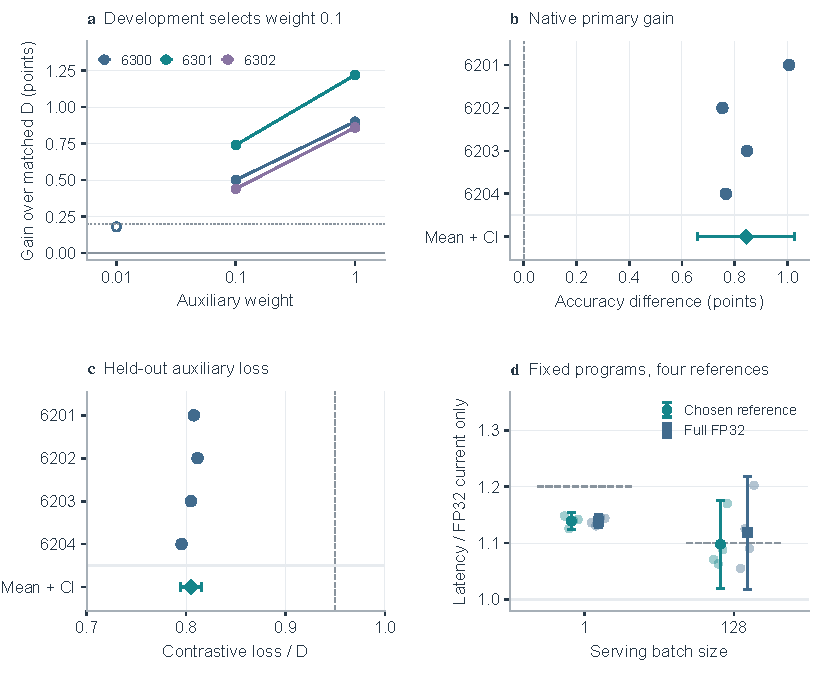
\includegraphics[width=\linewidth]{figures/fig_contrastive_benefit.pdf}
\caption{Visual auxiliary learning and native serving. (a) The smallest
weight meeting both development criteria is $0.1$. The open point marks
the $0.01$ pilot. (b) Native primary gain and (c) held-out contrastive
loss across four fitted references, averaging three continuations per
reference. The diamonds show means and $95\%$ intervals. (d) Forward
latency relative to the FP32 current program, using one endpoint per
reference. Dashed segments mark the fixed latency limits.}
\label{fig:contrastive_benefit}
\end{figure}
